\documentclass[12pt]{article}
\usepackage[top=1in, bottom=1in, left=1in, right=1in]{geometry}
\usepackage[french]{babel}

\usepackage[onehalfspacing]{setspace}

\usepackage{amsmath, amssymb, amsthm}
\usepackage{enumerate, enumitem}
\usepackage{fancyhdr, graphicx, proof, comment, multicol}
\usepackage[none]{hyphenat}
\usepackage{dirtytalk}
\binoppenalty=\maxdimen
\relpenalty=\maxdimen

\usepackage{microtype}
\usepackage{mathpazo}
\usepackage{mdframed}
\usepackage{parskip}
\linespread{1.1}
\usepackage{graphicx}
\usepackage{subfig}

\usepackage{mathrsfs}
\usepackage{amsfonts}
\usepackage{amsmath}
\usepackage{amssymb}

\usepackage{mathtools}
\newcommand{\defeq}{\vcentcolon=}
\newcommand{\eqdef}{=\vcentcolon}

\newenvironment{statement}[1]
{\begin{mdframed}[linewidth=0.6pt]
        \textsc{Statement #1:}

}

\newenvironment{ex}[1]
{\begin{mdframed}[linewidth=0.6pt]
        \textsc{Exercice #1:}

}
    {\end{mdframed}}

\newcommand{\R}{\mathbf{R}}
\newcommand{\C}{\mathbf{C}}
\newcommand{\Z}{\mathbf{Z}}
\newcommand{\N}{\mathbf{N}}
\newcommand{\Q}{\mathbf{Q}}

\newcommand{\de}{\mathrm{d}}

\newcommand*\quot[2]{{^{\textstyle #1}\big/_{\textstyle #2}}}

\theoremstyle{remark}
\newtheorem*{remark}{Remarque}
\newtheorem*{rap}{Rappel}

\begin{document}
        \noindent
\textbf{Systèmes dynamiques} \hfill \textbf{Vezin Lomàn}\\
\normalsize MAT551 \hfill Date de rendu: 20/10/2020\\

\begin{center}
\textbf{Devoir maison 4}
\end{center}
        
\begin{ex}{1}
        L'application angle de rotation \[
        \rho : (\mathrm{Homeo}(\quot{\R}{\Z}), D) \longmapsto \quot{\R}{\Z}
        \] est continue.
\end{ex}
\begin{proof}
        Soit $f$ un homéomorphisme du cercle et soit $F$ un relèvement. Soit $\varepsilon > 0$. Soit $g$ un autre homéomorphisme et $G$ un relèvement.

        Puisque $F, G$ sont des relèvements on a  \[
        \pi\circ F = f \circ\pi, \quad \text{et} \quad \pi\circ G = g \circ\pi
        .\] Ainsi en utilisant la surjectivité de la projection $\pi$,
        \begin{align*}
                D(f,g) &= \sup_{x\in\quot{\R}{\Z}}d(f(x), g(x)) \\
                       &= \sup_{x \in \R}d(f\circ\pi(x), g\circ\pi(x)) \\
                       &= \sup_{x\in \R}d(\pi\circ F(x),\pi\circ G(x)) \\
                       &= \sup_{x \in \R}\min_{\substack{\pi(X) = \pi(F(x)) \\ \pi(Y) = \pi(G(x))}}|X-Y| \\
                       &\ge \sup_{x \in [0,1]}\min_{\substack{\pi(X) = \pi(F(x)) \\ \pi(Y) = \pi(G(x))}}|X-Y| \\
                       &\ge \sup_{x \in [0,1]}\min_{p, q \in \Z}|F(x)+p-G(x)-q|
        .\end{align*}

        D'autre part comme $\phi_{F} \defeq F-Id$ et $\phi_{G} \defeq G-Id$ sont continues 1-périodiques on obtient
        \begin{align*}
                \|F-G\|_{\infty} &= \sup_{x\in\R}|F(x)-G(x)| \\
                                 &= \sup_{x\in\R}|F(x)-x-(G(x)-x)| \\
                                 &= \sup_{x\in [0,1]}|F(x)-G(x)| 
        .\end{align*}

        Comme les relèvements ne sont définis qu'à une constante entière près on en déduit \[
                D(f,g) \ge \|F-G\|_{\infty}
        ,\] pour un bon choix de $G$.

        On regarde à présent le nombre de rotation de $f$ et de $g$. Par convergence uniforme \[
                \frac{F^{k}-Id}{k} \to \rho(F) \quad \text{et} \quad \frac{G^{k}-Id}{k} \to \rho(G) 
        ,\] on a l'existence d'un rang $K > 0$ tel que pour tout $k \ge K$ \[
        |\frac{F^{k}(0)}{k} - \rho(F)| \le \frac{\varepsilon}{4} \quad \text{et} \quad |\frac{G^{k}(0)}{k} - \rho(G)| \le \frac{\varepsilon}{4} 
        .\] 

        En utilisant l'inégalité triangulaire on trouve
        \begin{align*}
                |\rho(F)-\rho(G)| &\le |\rho(F) - \frac{F^{k}(0)}{k}| + |\frac{F^{k}(0)-G^{k}(0)}{k}| + |\frac{G^{k}(0)}{k} - \rho(G)| \\
                                  &\le \frac{1}{k}\|F^{k}-G^{k}\|_{\infty} + \frac{\varepsilon}{2}
        .\end{align*}

        On montre que $F$ est uniformément continue, pour cela il suffit de remarquer que pour $x, y \in \R$ on a 
        \begin{align*}
                |F(x)-F(y)| &\le |F(x)-x+x-y+y-F(y)| \\
                            &\le |\phi_{F}(x) - \phi_{F}(y)| + |x-y|
        ,\end{align*} et le résultat découle de la continuité uniforme de $\phi_{F}$, continue et 1-périodique.

        Ainsi en utilisant encore une fois l'inégalité triangulaire,
        \begin{align*}
                \|F^{k}-G^{k}\|_{\infty} &\le \|F\circ F^{k-1} - F\circ G^{k-1}\|_{\infty} + \|F\circ G^{k-1} - G\circ G^{k-1}\| \\
                                         &\le \|F\circ F^{k-1} - F\circ G^{k-1}\|_{\infty} + \|F-G\|_{\infty} 
        .\end{align*}

        Puisque $F$ est uniformément continue $\|F^{k}-G^{k}\|_{\infty}$ est contrôlée par $\|F^{k-1}-G^{k-1}\|_{\infty}$, par itération directe $k$ fois, on peut alors trouver un $\delta > 0$ tel que pour $G$ satisfaisant $\|F-G\|_{\infty} < \delta$ on ait \[
                \|F^{k}-G^{k}\|_{\infty} \le \frac{k\varepsilon}{2}
        .\] 

        Il en découle alors directement que \[
                |\rho(F)-\rho(G)| \le \varepsilon
        .\]

        Ainsi lorsque $D(f,g)$ est assez petite on peut trouver $F, G$ deux relèvements respectivement de  $f, g$ satisfaisants  \[
                \|F-G\|_{\infty} \le D(f, g)
        .\] En prenant $D(f,g) \le \delta$ on obtient $|\rho(F)-\rho(G)| \le \varepsilon$, puisque le nombre de rotation d'un homéomorphisme n'est pas dépendant du choix de relèvement on en déduit 
        \[
                \lim_{D(f,g)\to 0}|\rho(f)-\rho(g)| = 0
        \]  ce qui garanti la continuité de $\rho$.
\end{proof}

\newpage

\begin{ex}{2}
        L'unique homéomorphisme affine par morceaux de $\quot{\R}{\Z}, \; f_{\lambda_1, \lambda_2}$ donné admet pour nombre de rotations
        \[
                \rho(f_{\lambda_1, \lambda_2}) = \frac{\log\lambda_1} {\log\lambda_1 -\log\lambda_2}
        .\] 
\end{ex}
\begin{proof}
        On se propose d'expliciter l'homéomorphisme en question. Si on note $b = f_{\lambda_1, \lambda_2}(0)$ on obtient 
        \begin{align*}
                f_{\lambda_1, \lambda_2}(x) = \begin{cases}
                        b+ \frac{1-b}{a}x, \quad &\text{si } 0 \le x < a \\
                        \frac{b}{1-a}(x-a), \quad &\text{si } a \le x < 1
                \end{cases}
        .\end{align*}
        On a alors bien $\lambda_1 = \frac{1-b}{a} > 1$ et $\lambda_2 = \frac{b}{1-a} < 1$. On propose une illustration ci dessous. 
        \begin{figure}[htpb]
                \centering
                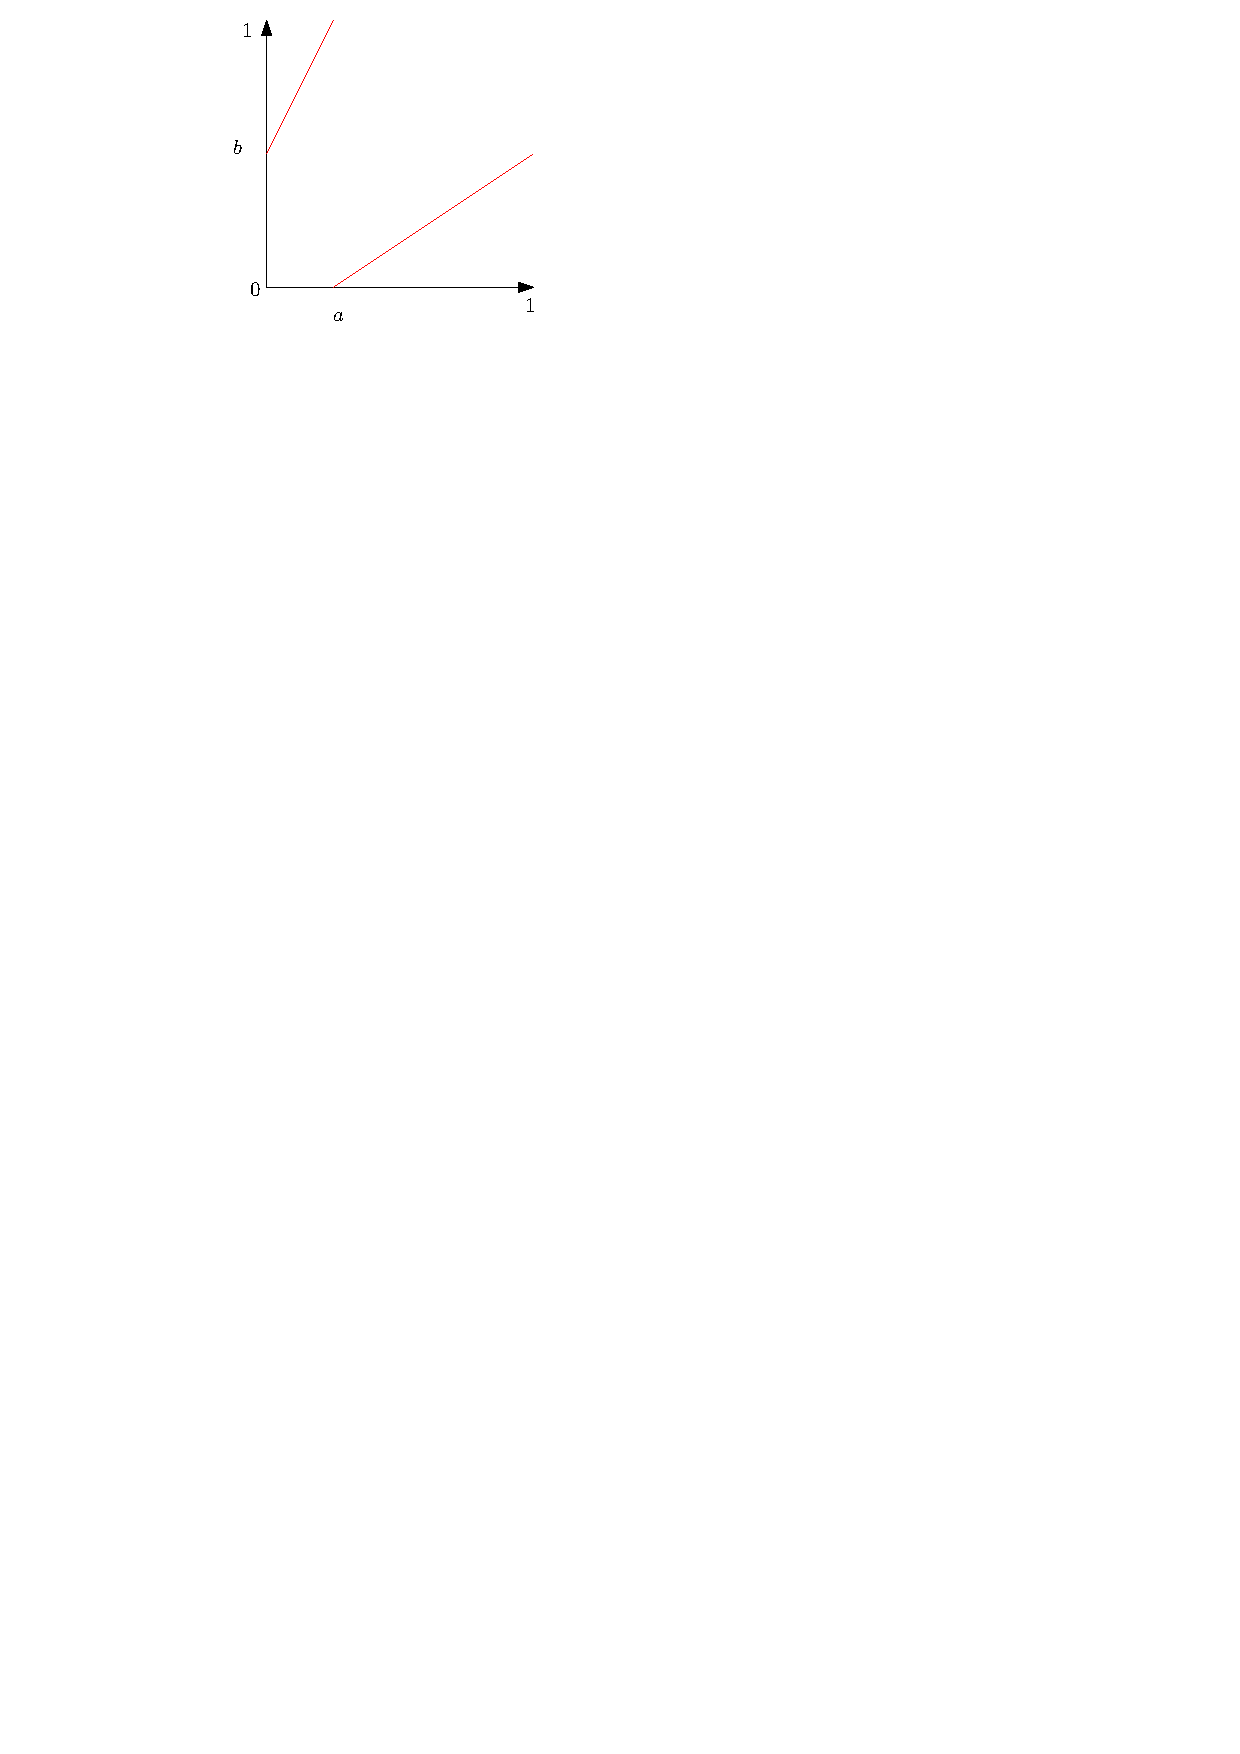
\includegraphics[width=0.4\textwidth]{homeo.pdf}
                \caption{Illustration du graphe de $f_{\lambda_1, \lambda_2}$}
                \label{fig:homeo-pdf}
        \end{figure}

        On pose $\sigma \defeq \frac{\lambda_1}{\lambda_2}$ et on considère l'homéomorphisme du cercle suivant
        \begin{align*}
                h : \quot{\R}{\Z} &\longmapsto \quot{\R}{\Z} \\
                x &\longmapsto \frac{\sigma^{x}-1}{\sigma-1} 
        .\end{align*}
        Cet homéomorphisme préserve l'orientation et un rapide calcul donne son inverse
        \begin{align*}
                h^{-1} : \quot{\R}{\Z} &\longmapsto \quot{\R}{\Z} \\
                y &\longmapsto \frac{\log(1+(\sigma -1)y)}{\log\sigma}
        .\end{align*}

        Un second calcul donne sur la première pente de $f_{\lambda_1, \lambda_2}$ 
        \begin{align*}
                h^{-1}\circ f_{\lambda_1, \lambda_2} \circ h (x) &= h^{-1} \circ f_{\lambda_1, \lambda_2} (\frac{\exp(x\log\sigma)}{\sigma-1})\\ 
                                                                 &= h^{-1}(b+\frac{1-b}{a}(\frac{\exp(x\log\sigma)}{\sigma-1})) \\
                                                                 &= \frac{1}{\log\sigma}\log[\frac{1}{a}(a+\sigma ab +b - ab + \sigma^{x} - 1-b\sigma^{x})]
        .\end{align*}

        Puis en se rappelant que \[
                \sigma = \frac{\lambda_1}{\lambda_2} = \frac{(1-b)(1-a)}{ab}
        ,\] on obtient
        \begin{align*}
                h^{-1}\circ f_{\lambda_1, \lambda_2} \circ h (x) &= \frac{1}{\log\sigma}\log[\frac{1-b}{a}\sigma^{x}] \\
                                                                 &= x + \frac{\log\frac{1-b}{a}}{\log\sigma}
        .\end{align*}
        Un calcul identique sur la deuxième pente de $f_{\lambda_1, \lambda_2}$ donne le même résultat. Ainsi $f_{\lambda_1, \lambda_2}$ est conjugué à une rotation d'angle \[
        \frac{\log(\frac{1-b}{a})}{\log\sigma} = \frac{\log\lambda_1} {\log\lambda_1 -\log\lambda_2}
        .\] L'angle d'une rotation correspond à son nombre de rotation, on sait que deux homéomorphismes conjugués ont le même nombre de rotation, on a donc le résultat.
\end{proof}

        \begin{remark}
                C'est un résultat intéressant puisqu'il montre qu'un homéomorphisme défini par des coefficients rationnels, même très simple, peut avoir un nombre de rotation irrationnel.
        \end{remark}
\end{document}
